\documentclass[12pt,a4paper]{article}

% -----------------------------------
% Подключение необходимых пакетов
% -----------------------------------
\usepackage[utf8]{inputenc}        % Кодировка UTF-8
\usepackage[T2A]{fontenc}          % Поддержка кириллицы
\usepackage[russian]{babel}        % Русский язык

\usepackage{graphicx}              % Вставка изображений
\usepackage{circuitikz}            % Рисование электрических схем

\title{Отчёт по выполнению КПЗ №1}
\author{Есиков С.Д, Иванова А. Я.}
\date{\today}

\begin{document}
	\maketitle
	\section{Задача}
	\begin{enumerate}
		\item Выбор конденсатора.
		\item Теоретические расчёты.
		\item Multisim-модель.
		\item АЧХ напряжения на ёмкости, индуктивности и тока в контуре.
		\item ПХ напряжений на ёмкости, индуктивности и тока в контуре.
		\item Декремент и частота собственных колебаний по ПХ.
		\item Добротность и частота резонанса по данным ПХ тока.
		\item Декремент и частота соственных колебаний по АЧХ.
		\item Исследование ПХ тока с внутренним сопротивлением источника
	\end{enumerate}
	\section{Условия}
	Был выбран вариант № 16, который соответствует следующим параметрам контура
	\begin{itemize}
		\item Ёмкость катушки ($L$) -- 470 мкГн
		\item Сопротвление катушки ($R_L$) -- 4 Ом
		\item Частота резонанса контура ($f_o$)-- 32 кГц
	\end{itemize}
	\newpage
	\section{Ход работы}
		\subsection{Выбор конденсатора.\newline}
		
			Вычислите ёмкость конденсатора, обеспечивающую резонанс на заданной частоте. 
			
			Выберите из ряда Е24 подходящую ёмкость.
			
			Полагаем: сопротивления потерь конденсатора и катушки одинаковые: $R_C = R_L$
			
			\medskip
			\medskip
			\medskip
			
			В соответствии с формулой $f_0 = \frac{1}{2\pi \cdot \sqrt{L \cdot C}}$ было получено, что
			
			\[C = \frac{1}{f_0^2 \cdot L} = \frac{1}{4\pi^2 \cdot 3.2^2 \cdot 4.7 \cdot 10^4} = 5.18\cdot 10^{-8} F = 51.8 \eta F\]
			
			\medskip
			\medskip
			
			Номинальный ряд Е24 содержит слеюущие номиналы
			
				\begin{tabular}{|c|c|c|c|c|c|c|c|c|c|c|c|c|c|c|c|c|c|c|c|c|c|c|c|c|}
						\hline
						E24 & 1.0 & 1.1 & 1.2 & 1.3 & 1.5 & 1.6 & 1.8 & 2.0 & 2.2 & 2.4 & 2.7 & 3.0 \\
						\hline
						& 3.3 & 3.6 & 3.9 & 4.3 & 4.7 & 5.1 & 5.6 & 6.2 & 6.8 & 7.5 & 8.2 & 9.1	\\
						\hline
				\end{tabular}
			
			\medskip
			\medskip
			
			Учитывая что требуется подобрать ёмкость, так чтобы частота была максимально близкой к заданной слева, ёмкость следует выбирать максимально близкой к требуёмой справа - $5.6 \cdot 10^{-8}$ Ф (56 нФ)
			
			\[C = 56 \eta F\]
			 
		\newpage
		
		\subsection{Теоретические расчёты.\newline}
		
		Вычислите частоту резонанса, добротность контура, ширину резонансной характеристики тока и её отношение к частоте резонанса (сопоставьте с 1/Q)
		
		Частота резонанса
		
		\[f = \frac{1}{2\pi \cdot \sqrt{L \cdot C}} = \frac{1}{2\pi \cdot \sqrt{4.7 \cdot 5.6 \cdot 10^{-12}}} = 31021.5 \ Hz = 31.021 \ kHz\]
		
		Добротность конутра
		
		\[Q = \frac{\sqrt{L \cdot C}}{2R_L} = \frac{\sqrt{4.7 \cdot 10^4 / 5.6 }}{2 \cdot 4} = 11.451\]
		
		Отношение добротности к частоте резонанса
		
		\[\frac{Q}{f} = \frac{11.451}{31021.5} = 3.691 \cdot 10^{-4}\]
		
		\medskip
		\medskip
		
		
		\subsection{Multisim-модель.\newline}
			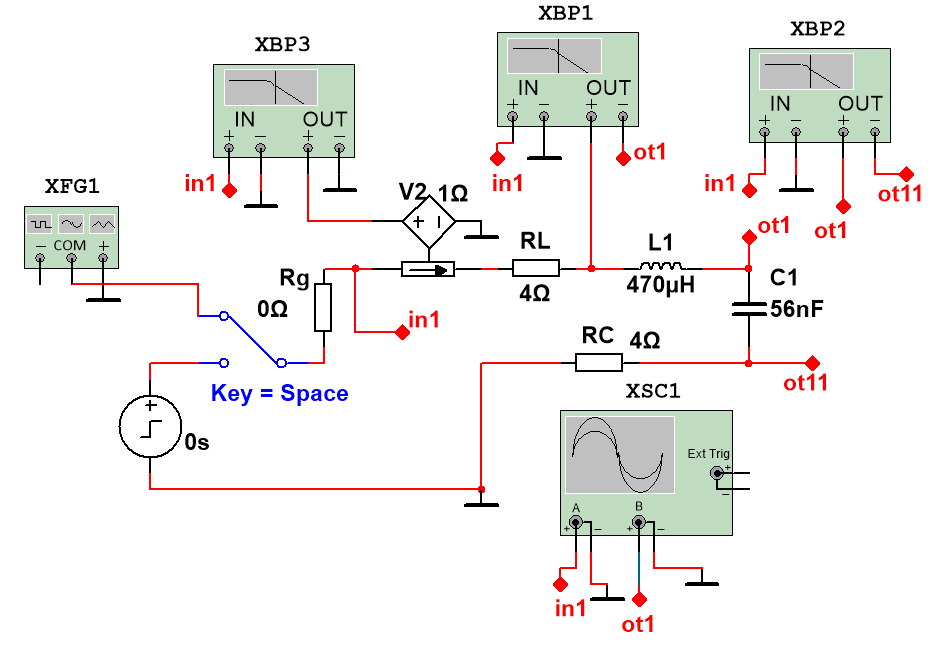
\includegraphics[width=\linewidth]{src/model}
			\label{fig:model}

		\newpage
		
		\subsection{АЧХ напряжения на ёмкости, индуктивности и тока в контуре.\newline}	
		
			Исследуйте плоттером Боде АЧХ напряжения на ёмкости, индуктивности и АЧХ тока в контуре.
			Выясните: 
			
			значения частот в максимумах АЧХ;
			
			относительную ширину резонансной кривой тока и по ней добротность контура.
			
						
			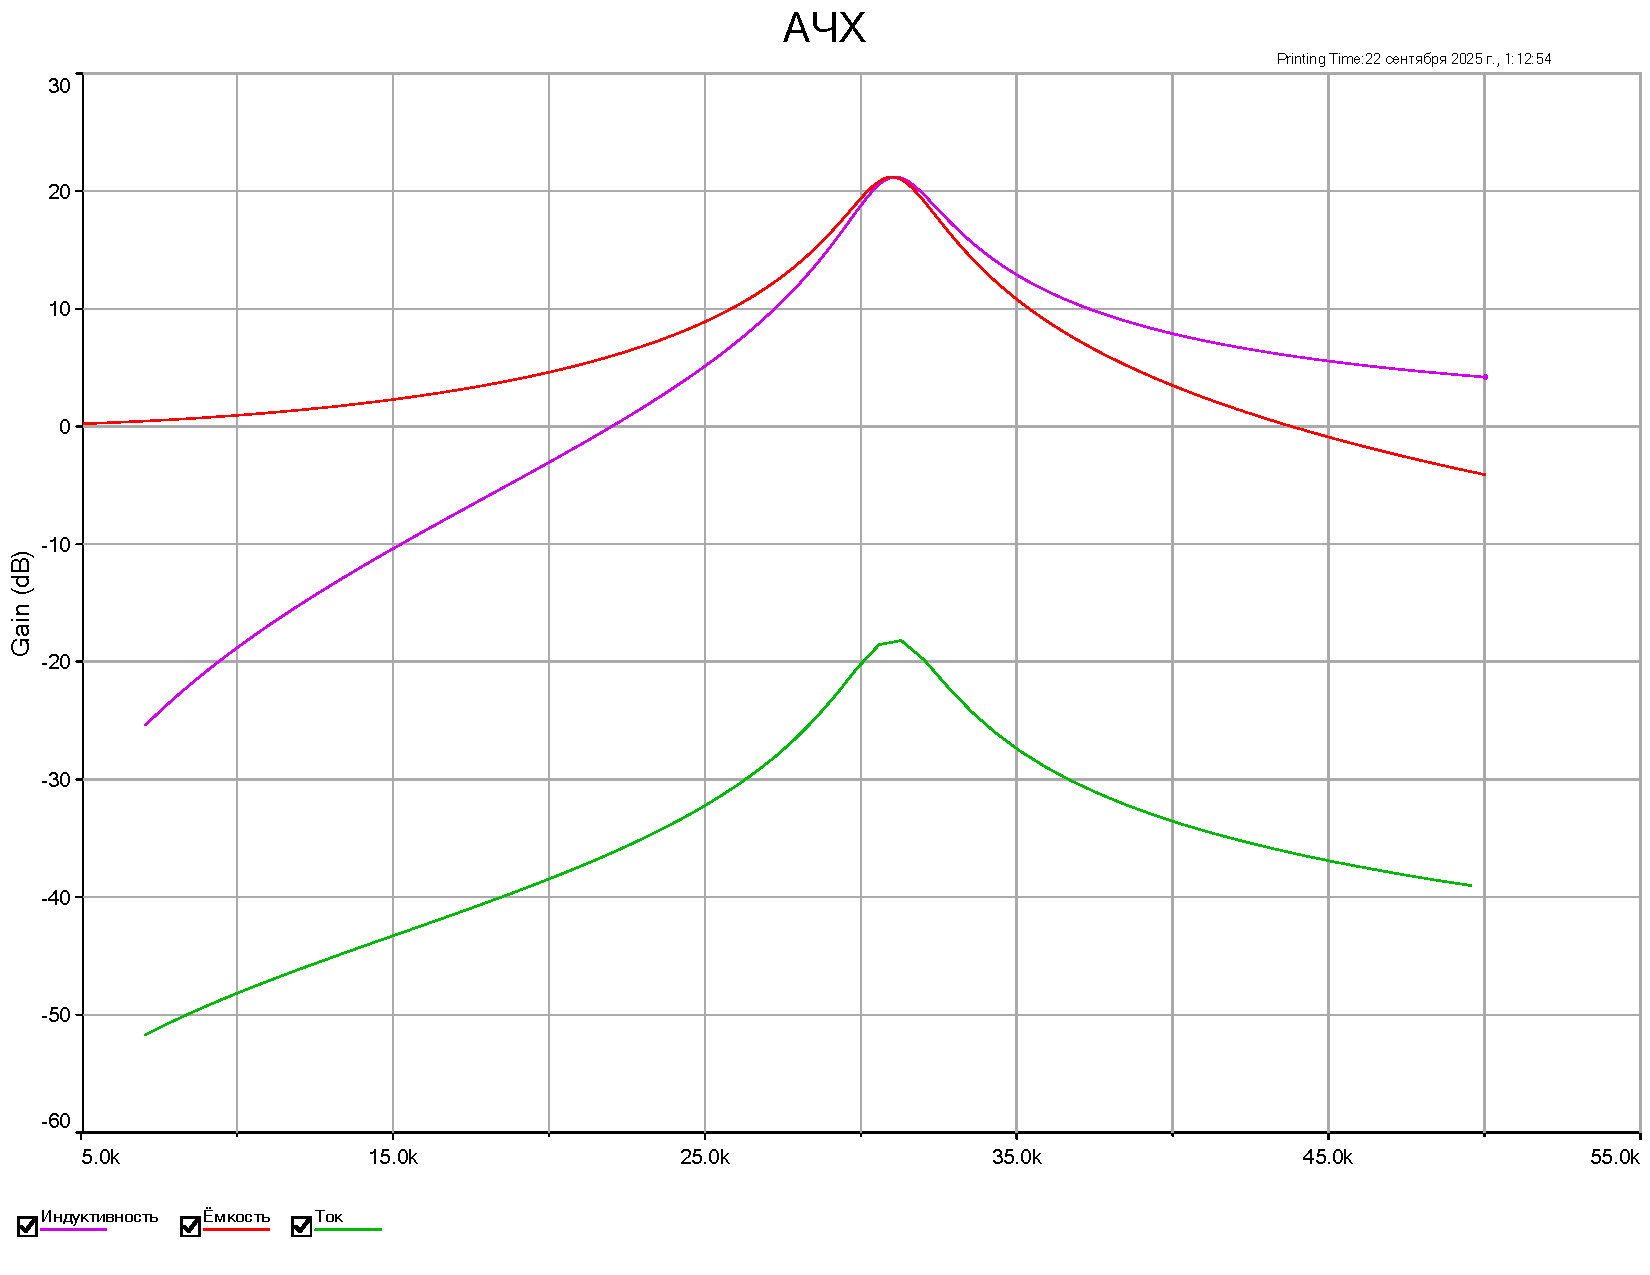
\includegraphics[width=\linewidth]{src/MFH}

			\newpage
	
			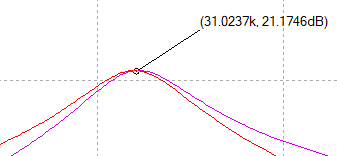
\includegraphics[width=0.5\linewidth]{src/MFH_max_1}
			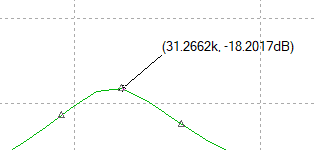
\includegraphics[width=0.5\linewidth]{src/MFH_max_2}
			
			Как видно максимумы аплитуд приходятся примерно на 31 кГц
		
			Чтобы посчитать относительную ширину резонансной кривой, нужно взять 70\% от амплитуды и изменить разност частоть
			
			В нашем случае амплитуда составляет примерно 20 dB значит нужно спуститься на 6 db от -18, то есть -24 dB
			
			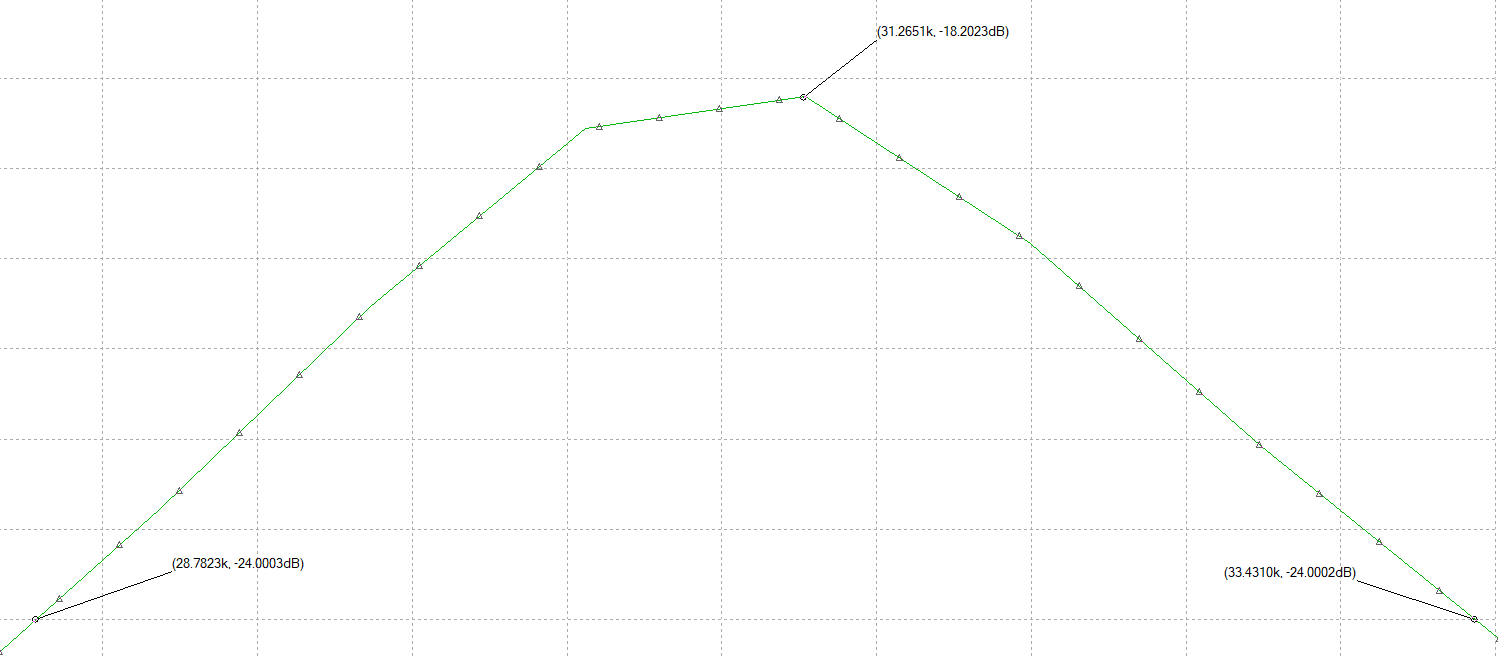
\includegraphics[width=1\linewidth]{src/MFH_current_weight}
			
			Выходит, что ширина равна приерно 33.431 - 28.7823 = 4.6487 кГц
			
			Добротность тогда выходит 31.2651 / 4.6487 = 6.725, что на полпорядка отличается от добротности полученной при расчётах
			
			\newpage			

		\subsection{ПХ напряжений на ёмкости, индуктивности и тока в контуре.\newline}
		
			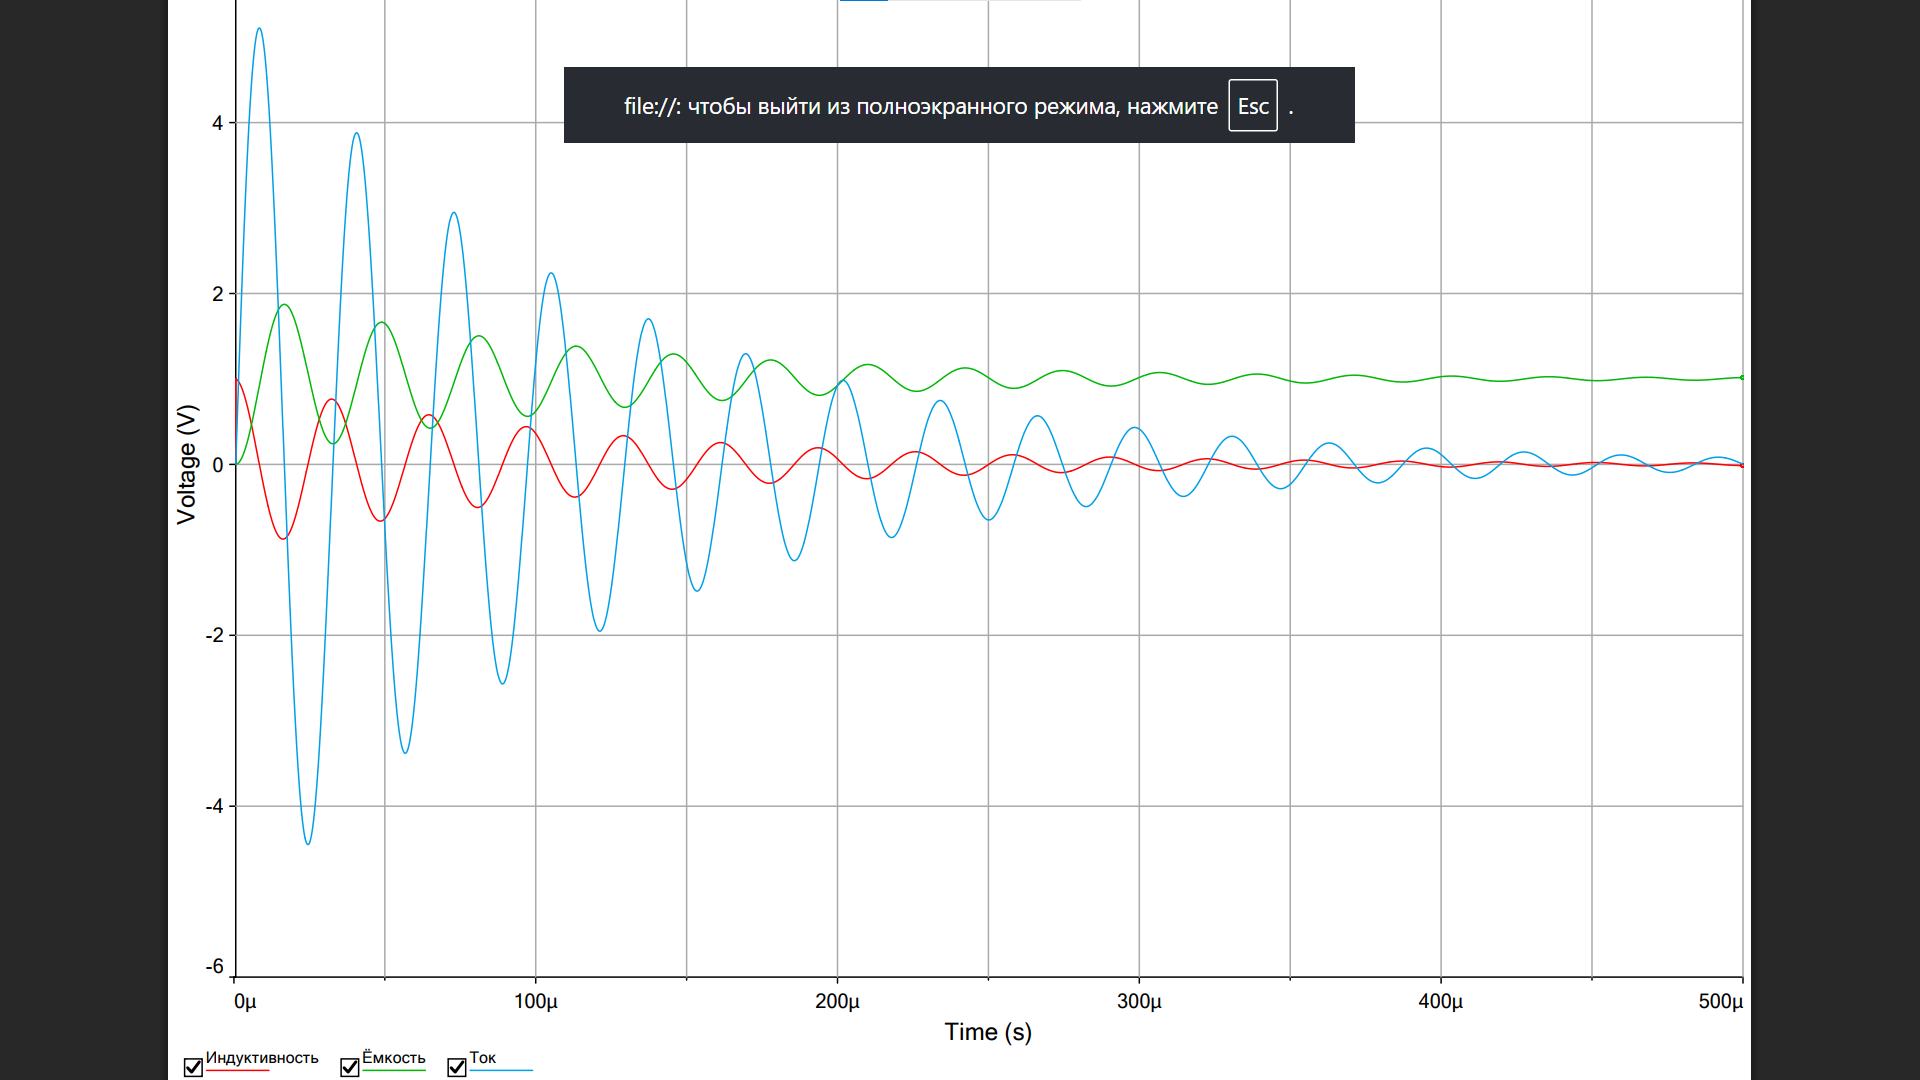
\includegraphics[width=1\linewidth]{src/TH}

		\newpage
		
		\subsection{Декремент и частота собственных колебаний по ПХ.\newline}
		
			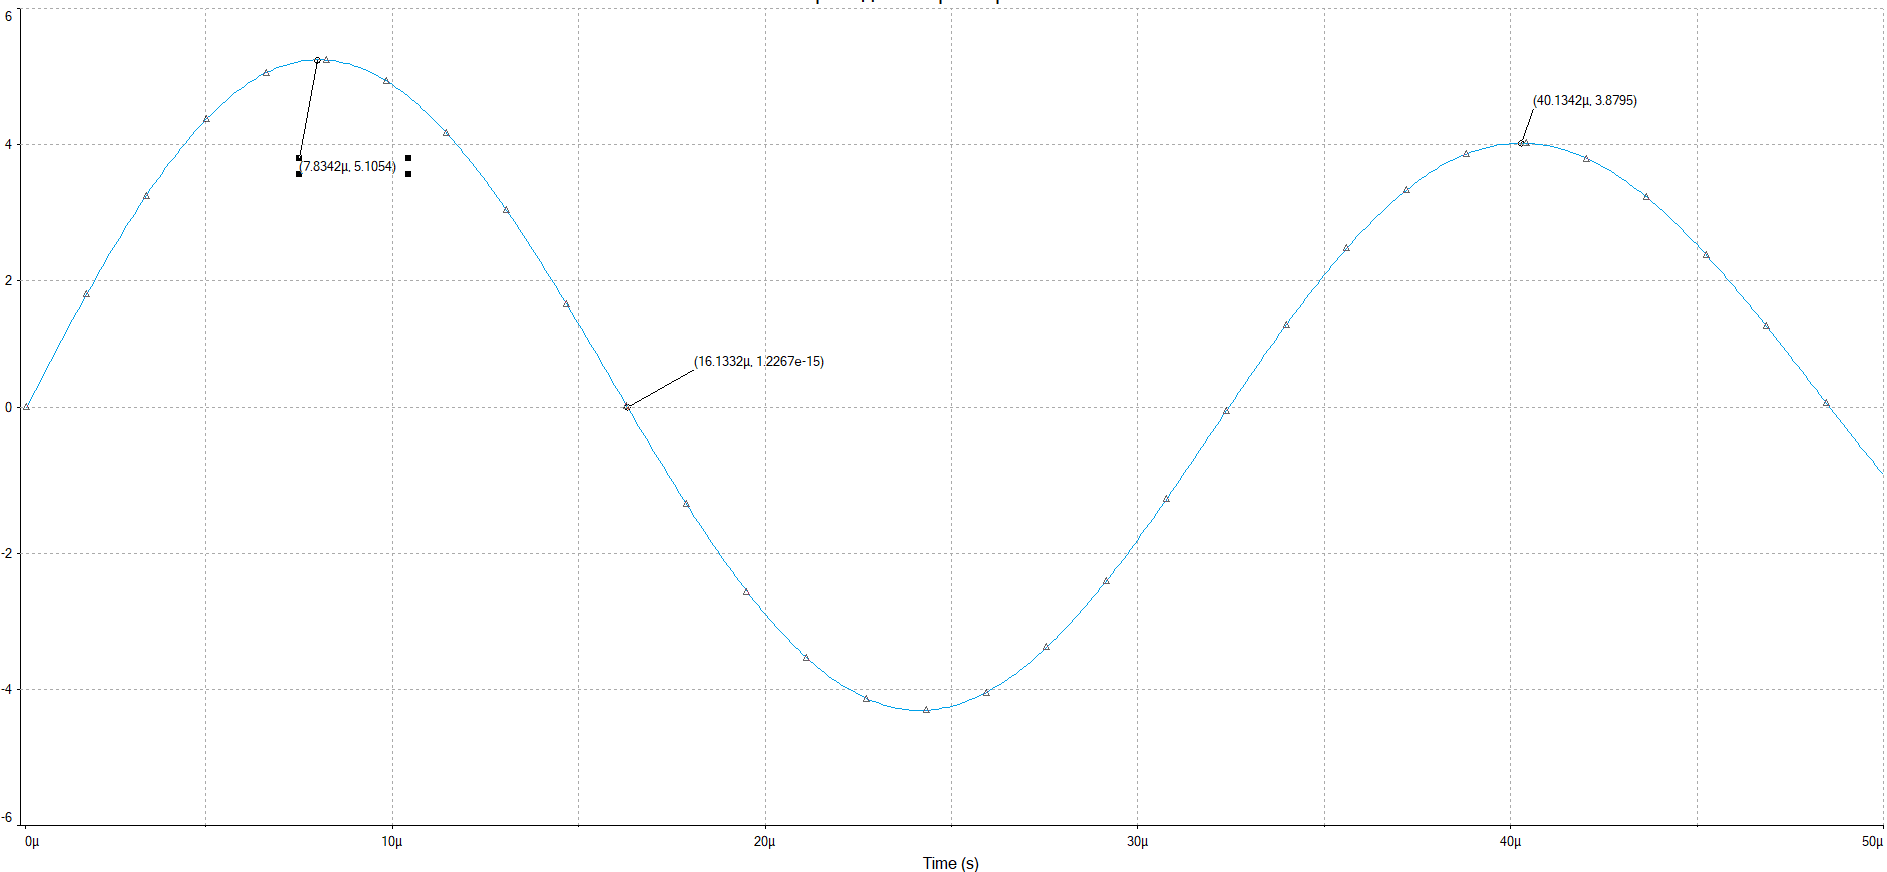
\includegraphics[width=1\linewidth]{src/TH_current}
			
			Декремент считается как отношение двух соседних амплитуд колебаний (в силу симметричности графика относительно нуля, можно брать отношение полуамплитуд, то есть значений в пиках)
			
			Тогда декремент будет $ln\left(\frac{5.1054}{3.8795}\right) = 0.275$

			Частоту считаем как половину от обратного к полупериоду
			
			\[\frac{0.5}{16.1322 \cdot 10^{-6}} = 31006.2 Hz = 31.006 kHz\]
			
		\subsection{Добротность и частота резонанса по данным ПХ тока.\newline}
			
			\[Q = \frac{\pi}{\delta} = \frac{\pi}{0.275} = 11.424\]
			
			Резонансной же частотой будет вычисленная ранее частота собственных колебаний --- 31.006 кГц
			
		\subsection{Декремент и частота соственных колебаний по АЧХ.\newline}
		
			\[\delta = \frac{\pi}{Q} = \frac{\pi}{6.725} = 0.4659; f = 31.265 kHz\]
			
		\subsection{Исследование ПХ тока с внутренним сопротивлением источника\newline}
		
			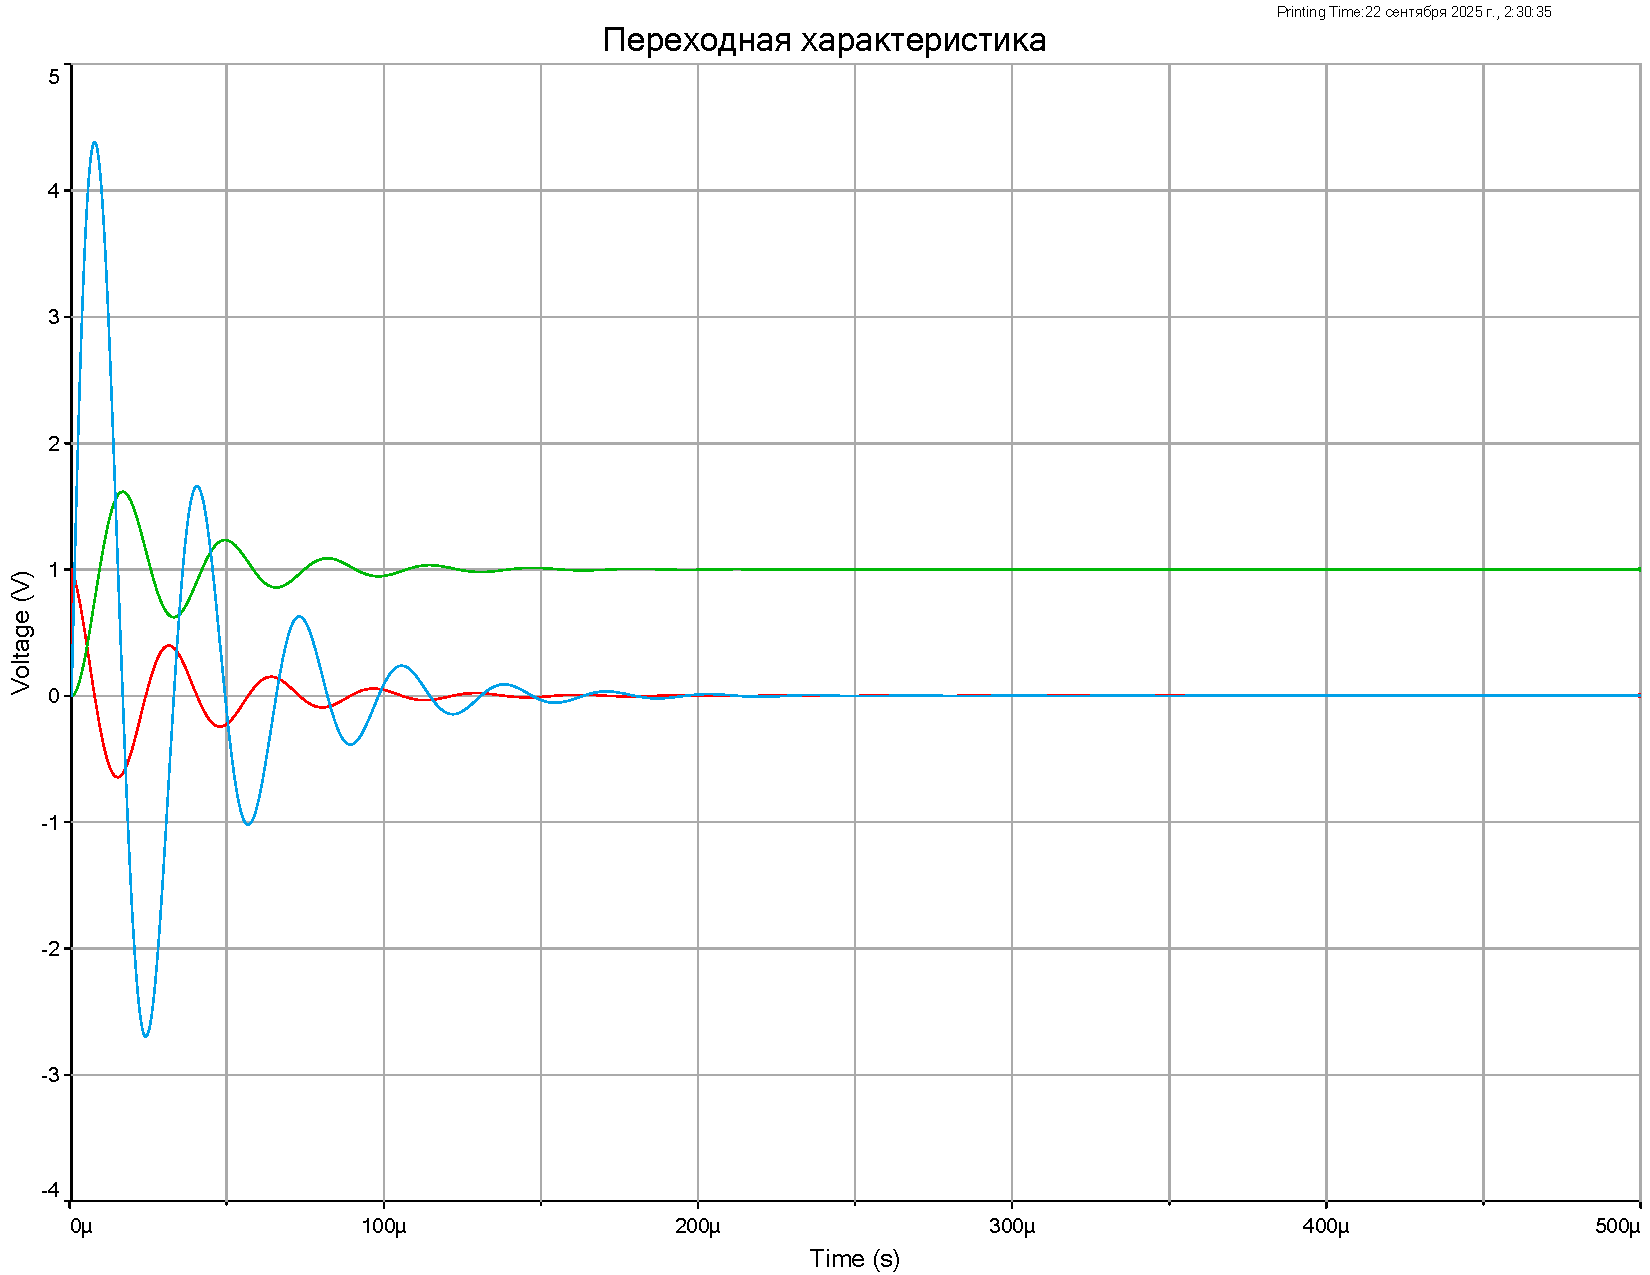
\includegraphics[width=0.5\linewidth]{src/TH_20om}
			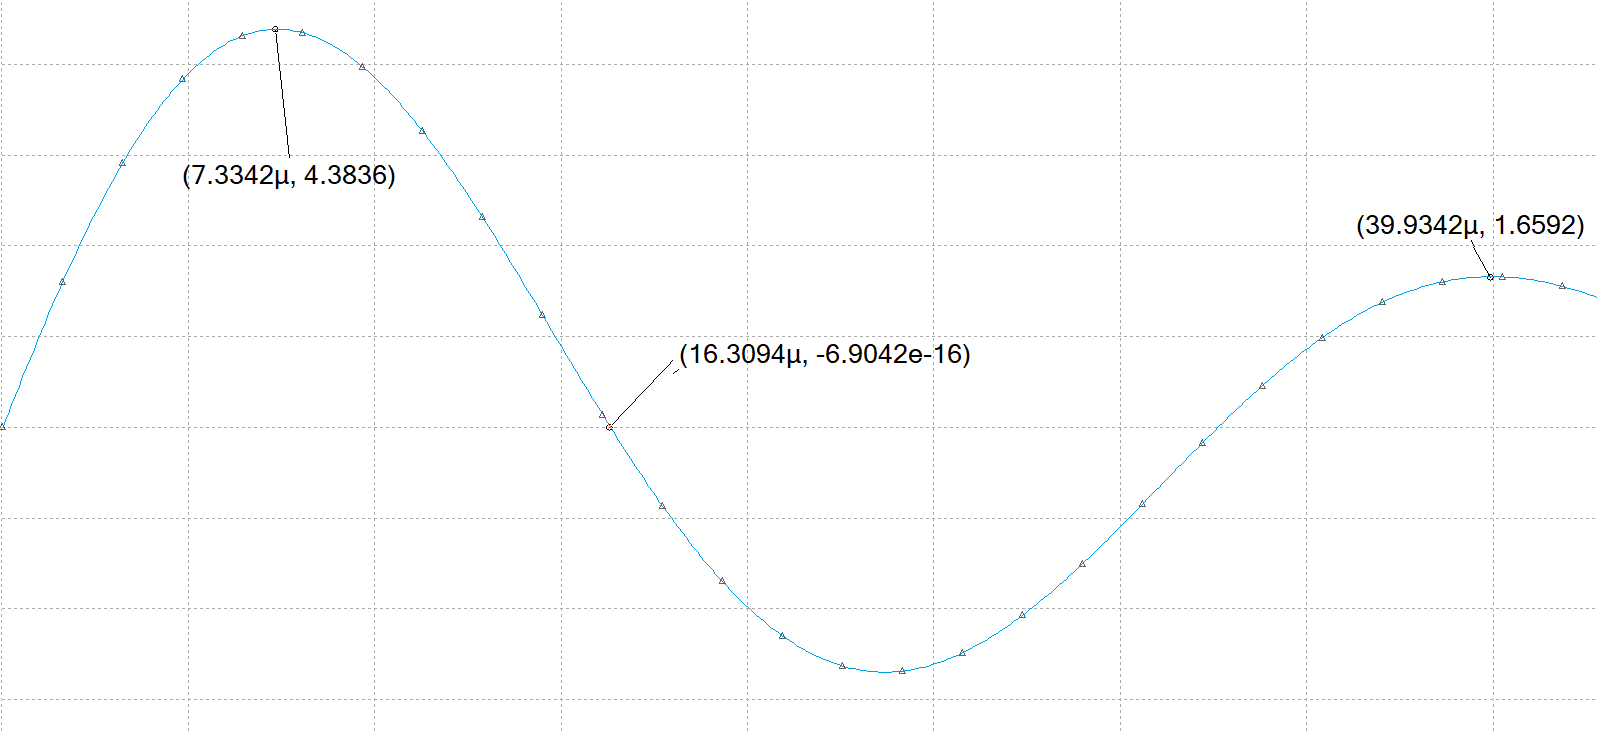
\includegraphics[width=0.5\linewidth]{src/TH_current_20m}
			
			\[\delta = ln\left(\frac{4.3836}{1.6592}\right) = 0.971\]
			
			\[f = \frac{0.5}{16.3094 \cdot 10^{-6}} = 30657 Hz = 30.657 kHz\]
			
			\[Q = \frac{\pi}{\delta} = \frac{\pi}{0.971} = 3.236\]
			
		\subsection{Сравнение результатов}
		
		\centering
		\begin{tabular}{|c|c|c|c|c|}
			\hline
			Переменая & По расчётам & по АЧХ & по ПХ & по ПХ с потерями \\
			\hline
			f & 31.021 kHz & 31.265 kHz & 31.006 kHz & 30.657 kHz \\
 			\hline
			Q & 11.451 & 6.725 & 11.424 & 3.236 \\
			\hline
			$\delta$ & 0.274 & 0.4659 & 0.275 & 0.971 \\
			\hline
		\end{tabular}
		
		\newpage
		
		\section{Заключение}
		
		До сих пор для нас остаётся загадкой то, почему значения добротности и дикремента по АЧХ настолько отличаются от расчётных, основное предположение - прямая зависимость этих значений от выбираемой частотной ширины
		
		В остальном все значения получились достаточно близкими к расчётным, что говорит о правильно проведёных расчётах и корректно поставленном исследовании реальной модели
		
		Видно что внутреннее сопротивление источника с одной стороны не оказывает больших изменений на резонансную частоту контура, что хорошо в рамках работы частотных фильтров, однако кратно увеличивает потери энергии, что снижает помехоустойчивость, но при этом увелчивает ширину воспринимаемой конутром частоты
\end{document}	